
\documentclass[11pt,compress,t,notes=noshow, xcolor=table]{beamer}
\usepackage[]{graphicx}\usepackage[]{color}
% maxwidth is the original width if it is less than linewidth
% otherwise use linewidth (to make sure the graphics do not exceed the margin)
\makeatletter
\def\maxwidth{ %
  \ifdim\Gin@nat@width>\linewidth
    \linewidth
  \else
    \Gin@nat@width
  \fi
}
\makeatother

\definecolor{fgcolor}{rgb}{0.345, 0.345, 0.345}
\newcommand{\hlnum}[1]{\textcolor[rgb]{0.686,0.059,0.569}{#1}}%
\newcommand{\hlstr}[1]{\textcolor[rgb]{0.192,0.494,0.8}{#1}}%
\newcommand{\hlcom}[1]{\textcolor[rgb]{0.678,0.584,0.686}{\textit{#1}}}%
\newcommand{\hlopt}[1]{\textcolor[rgb]{0,0,0}{#1}}%
\newcommand{\hlstd}[1]{\textcolor[rgb]{0.345,0.345,0.345}{#1}}%
\newcommand{\hlkwa}[1]{\textcolor[rgb]{0.161,0.373,0.58}{\textbf{#1}}}%
\newcommand{\hlkwb}[1]{\textcolor[rgb]{0.69,0.353,0.396}{#1}}%
\newcommand{\hlkwc}[1]{\textcolor[rgb]{0.333,0.667,0.333}{#1}}%
\newcommand{\hlkwd}[1]{\textcolor[rgb]{0.737,0.353,0.396}{\textbf{#1}}}%
\let\hlipl\hlkwb

\usepackage{framed}
\makeatletter
\newenvironment{kframe}{%
 \def\at@end@of@kframe{}%
 \ifinner\ifhmode%
  \def\at@end@of@kframe{\end{minipage}}%
  \begin{minipage}{\columnwidth}%
 \fi\fi%
 \def\FrameCommand##1{\hskip\@totalleftmargin \hskip-\fboxsep
 \colorbox{shadecolor}{##1}\hskip-\fboxsep
     % There is no \\@totalrightmargin, so:
     \hskip-\linewidth \hskip-\@totalleftmargin \hskip\columnwidth}%
 \MakeFramed {\advance\hsize-\width
   \@totalleftmargin\z@ \linewidth\hsize
   \@setminipage}}%
 {\par\unskip\endMakeFramed%
 \at@end@of@kframe}
\makeatother

\definecolor{shadecolor}{rgb}{.97, .97, .97}
\definecolor{messagecolor}{rgb}{0, 0, 0}
\definecolor{warningcolor}{rgb}{1, 0, 1}
\definecolor{errorcolor}{rgb}{1, 0, 0}
\newenvironment{knitrout}{}{} % an empty environment to be redefined in TeX

\usepackage{alltt}
\newcommand{\SweaveOpts}[1]{}  % do not interfere with LaTeX
\newcommand{\SweaveInput}[1]{} % because they are not real TeX commands
\newcommand{\Sexpr}[1]{}       % will only be parsed by R
\newcommand{\xmark}{\ding{55}}%


\usepackage[english]{babel}
\usepackage[utf8]{inputenc}

\usepackage{dsfont}
\usepackage{verbatim}
\usepackage{amsmath}
\usepackage{amsfonts}
\usepackage{amssymb}
\usepackage{bm}
\usepackage{csquotes}
\usepackage{multirow}
\usepackage{longtable}
\usepackage{booktabs}
\usepackage{enumerate}
\usepackage[absolute,overlay]{textpos}
\usepackage{psfrag}
\usepackage{algorithm}
\usepackage{algpseudocode}
\usepackage{eqnarray}
\usepackage{arydshln}
\usepackage{tabularx}
\usepackage{placeins}
\usepackage{tikz}
\usepackage{setspace}
\usepackage{colortbl}
\usepackage{mathtools}
\usepackage{wrapfig}
\usepackage{bm}
\usepackage{amsmath}
\usepackage{pifont}
\usepackage{xcolor} %colored math symbols

\usetikzlibrary{shapes,arrows,automata,positioning,calc,chains,trees, shadows}
\tikzset{
  %Define standard arrow tip
  >=stealth',
  %Define style for boxes
  punkt/.style={
    rectangle,
    rounded corners,
    draw=black, very thick,
    text width=6.5em,
    minimum height=2em,
    text centered},
  % Define arrow style
  pil/.style={
    ->,
    thick,
    shorten <=2pt,
    shorten >=2pt,}
}

\usepackage{subfig}

% Defines macros and environments
\usepackage{../../style/lmu-lecture}


\let\code=\texttt
\let\proglang=\textsf

\setkeys{Gin}{width=0.9\textwidth}

\setbeamertemplate{frametitle}{\expandafter\uppercase\expandafter\insertframetitle}

\usepackage{bbm}
% basic latex stuff
\newcommand{\pkg}[1]{{\fontseries{b}\selectfont #1}} %fontstyle for R packages
\newcommand{\lz}{\vspace{0.5cm}} %vertical space
\newcommand{\dlz}{\vspace{1cm}} %double vertical space
\newcommand{\oneliner}[1] % Oneliner for important statements
{\begin{block}{}\begin{center}\begin{Large}#1\end{Large}\end{center}\end{block}}


%new environments
\newenvironment{vbframe}  %frame with breaks and verbatim
{
 \begin{frame}[containsverbatim,allowframebreaks]
}
{
\end{frame}
}

\newenvironment{vframe}  %frame with verbatim without breaks (to avoid numbering one slided frames)
{
 \begin{frame}[containsverbatim]
}
{
\end{frame}
}

\newenvironment{blocki}[1]   % itemize block
{
 \begin{block}{#1}\begin{itemize}
}
{
\end{itemize}\end{block}
}

\newenvironment{fragileframe}[2]{  %fragile frame with framebreaks
\begin{frame}[allowframebreaks, fragile, environment = fragileframe]
\frametitle{#1}
#2}
{\end{frame}}


\newcommand{\myframe}[2]{  %short for frame with framebreaks
\begin{frame}[allowframebreaks]
\frametitle{#1}
#2
\end{frame}}

\newcommand{\remark}[1]{
  \textbf{Remark:} #1
}


\newenvironment{deleteframe}
{
\begingroup
\usebackgroundtemplate{
\includegraphics[width=\paperwidth,height=\paperheight]{../style/color/red.png}}
 \begin{frame}
}
{
\end{frame}
\endgroup
}
\newenvironment{simplifyframe}
{
\begingroup
\usebackgroundtemplate{
\includegraphics[width=\paperwidth,height=\paperheight]{../style/color/yellow.png}}
 \begin{frame}
}
{
\end{frame}
\endgroup
}\newenvironment{draftframe}
{
\begingroup
\usebackgroundtemplate{
\includegraphics[width=\paperwidth,height=\paperheight]{../style/color/green.jpg}}
 \begin{frame}
}
{
\end{frame}
\endgroup
}
% https://tex.stackexchange.com/a/261480: textcolor that works in mathmode
\makeatletter
\renewcommand*{\@textcolor}[3]{%
  \protect\leavevmode
  \begingroup
    \color#1{#2}#3%
  \endgroup
}
\makeatother


\input{../../latex-math/basic-math}
\input{../../latex-math/basic-ml}
\input{../../latex-math/ml-nn}

\newcommand{\titlefigure}{plots/attention3.png}
%modify picture
\newcommand{\learninggoals}{
  \item Familiarize with the most recent sequence data modeling technique:
\begin{itemize}
\item \footnotesize Attention Mechanism
  \item \footnotesize Transformers
\end{itemize}
  \item Get to know the CNN alternative to RNNs
}

\title{Deep Learning}
\date{}



\begin{document}

\lecturechapter{Attention and Transformers}
\lecture{I2DL}

%%%%%%%%%%%%%%%%%%%%%%%%%%%%%%%%%%%%%%%%%%%%%%%%%%%%%%%%%%%%%%%%%%
%%%%%%%%%%%%%%%%%%%%%%%%%%%%%%%%%%%%%%%%%%%%%%%%%%%%%%%%%%%%%%%%%%

\section{Attention}

\begin{vbframe}{Attention}
  \begin{itemize}
    \item In a classical decoder-encoder RNN all information about the input sequence must be incorporated into the final hidden state, which is then passed as an input to the decoder network.
    \item With a long input sequence this fixed-sized context vector is unlikely to capture all relevant information about the past.
      \item Each hidden state contains mostly information from recent inputs. 
      %In the case of a bidirectional RNN to encode the input sequence, a hidden state contains information from recent preceding and following inputs.
      \item Key idea: Allow the decoder to access all the hidden states of the encoder (instead of just the final one) so that it can dynamically decide which ones are relevant at each time-step in the decoding.
      \item This means the decoder can choose to "focus" on different hidden states (of the encoder) at different time-steps of the decoding process similar to how the human eye can focus on different regions of the visual field.
      \item This is known as an \textbf{attention mechanism}.
   \end{itemize}
   
   \framebreak
   
   \begin{itemize}
      \item The attention mechanism is implemented by an additional component in the decoder.
      \item For example, this can be a simple single-hidden layer feed-forward neural network which is trained along with the RNN.
      \item At any given time-step $i$ of the decoding process, the network computes the relevance of encoder state $\mathbf{z}^{[j]}$ as:
            $$ rel(\mathbf{z}^{[j]})^{[i]} = \mathbf{v}_a^\top \text{tanh} (\mathbf{W}_a[\mathbf{g}^{[i-1]};\mathbf{z}^{[j]}]) $$
            where $\mathbf{v}_a$ and $\mathbf{W}_a$ are the parameters of the feed-forward network, $\mathbf{g}^{[i-1]}$ is the decoder state from the previous time-step and ';' indicates concatenation.
      %\item $v_a$ and $W_a$ are also learned through backpropagation.
      \item The relevance scores (for all the encoder hidden states) are then normalized which gives the \textit{attention weights} $(\alpha^{[j]})^{[i]}$:      
        $$ (\alpha^{[j]})^{[i]} = \frac{\exp (rel(\mathbf{z}^{[j]})^{[i]})}{\sum_{j'} \exp(rel(\mathbf{z}^{[j']})^{[i]})} $$
   \end{itemize}
   
   \framebreak
   
   \begin{itemize}  
    \item The attention mechanism allows the decoder network to focus on different parts of the input sequence by adding connections from all hidden states of the encoder to each hidden state of the decoder.
  %  \item At each point in time, a set of weights is computed which determine how to combine the hidden states of the encoder into a context vector $c_i$, which holds the necessary information to predict the correct output.
 %   \item Each hidden state contains mostly information from recent inputs. In the case of a bidirectional RNN to encode the input sequence, a hidden state contains information from recent preceding and following inputs.
  \end{itemize}
 \begin{figure}
    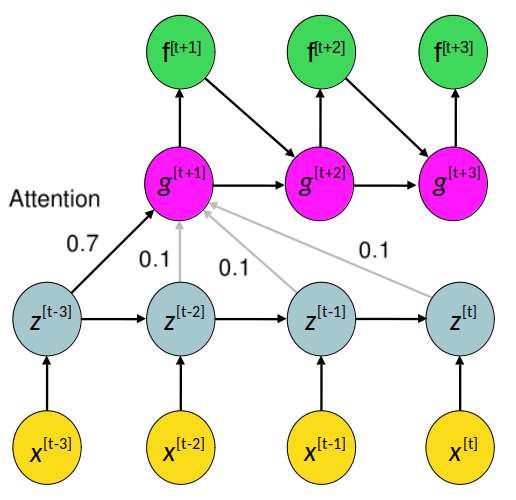
\includegraphics[width=5.cm]{figure/seq2seq_3.png}
    \caption{Attention at $i=t+1$}
  \end{figure}
 
\framebreak
\begin{itemize}  
   % \item An \textbf{attention mechanism} allows the decoder network to focus on different parts of the input sequence by adding connections from all hidden states of the encoder to each hidden state of the decoder
    \item At each time step $i$, a set of weights $(\alpha^{[j]})^{[i]}$ is computed which determine how to combine the hidden states of the encoder into a context vector $\mathbf{g}^{[i]}= \sum_{j=1}^{n_x} (\alpha^{[j]})^{[i]} \mathbf{z}^{[j]}$, which holds the necessary information to predict the correct output.
 %   \item Each hidden state contains mostly information from recent inputs. In the case of a bidirectional RNN to encode the input sequence, a hidden state contains information from recent preceding and following inputs.
  \end{itemize}
  \begin{figure}
    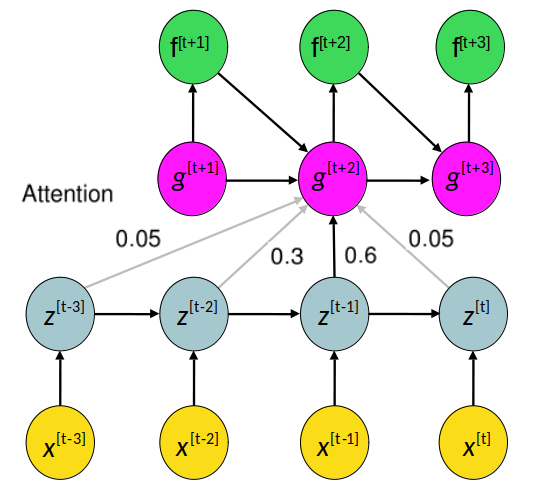
\includegraphics[width=5.cm]{figure/seq2seq_4.png}
    \caption{Attention at $i=t+2$}
  \end{figure}
  
\framebreak
  
  \lz
  \lz
  \begin{figure}
    \centering
    \scalebox{0.9}{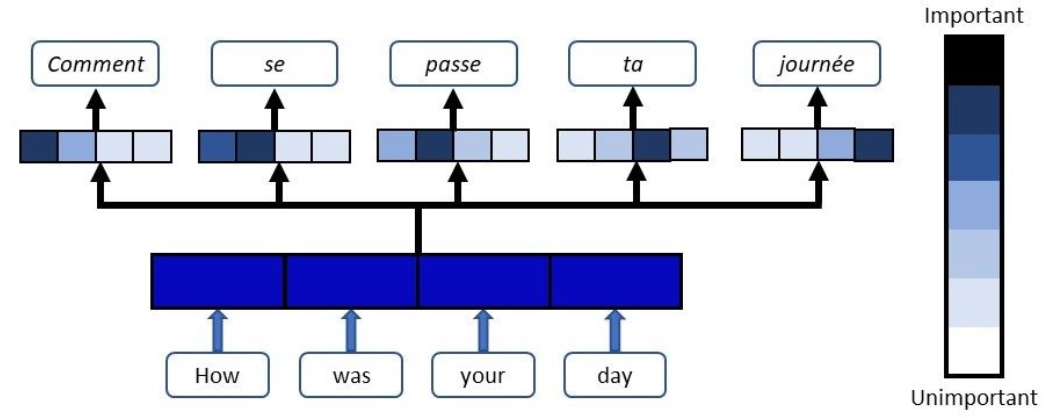
\includegraphics{plots/attention_example.png}}
    \tiny{\\Credit: Gabriel Loye}
    \caption{\footnotesize An illustration of a machine translation task using an encoder-decoder model with an attention mechanism. The attention weights at each time-step of the decoding/translation process indicate which parts of the input sequence are most relevant. (There are 4 attention weights because there are 4 encoder states.)}
  \end{figure}
  
  
\end{vbframe}

\frame{
\frametitle{Attention}
  \begin{figure}
    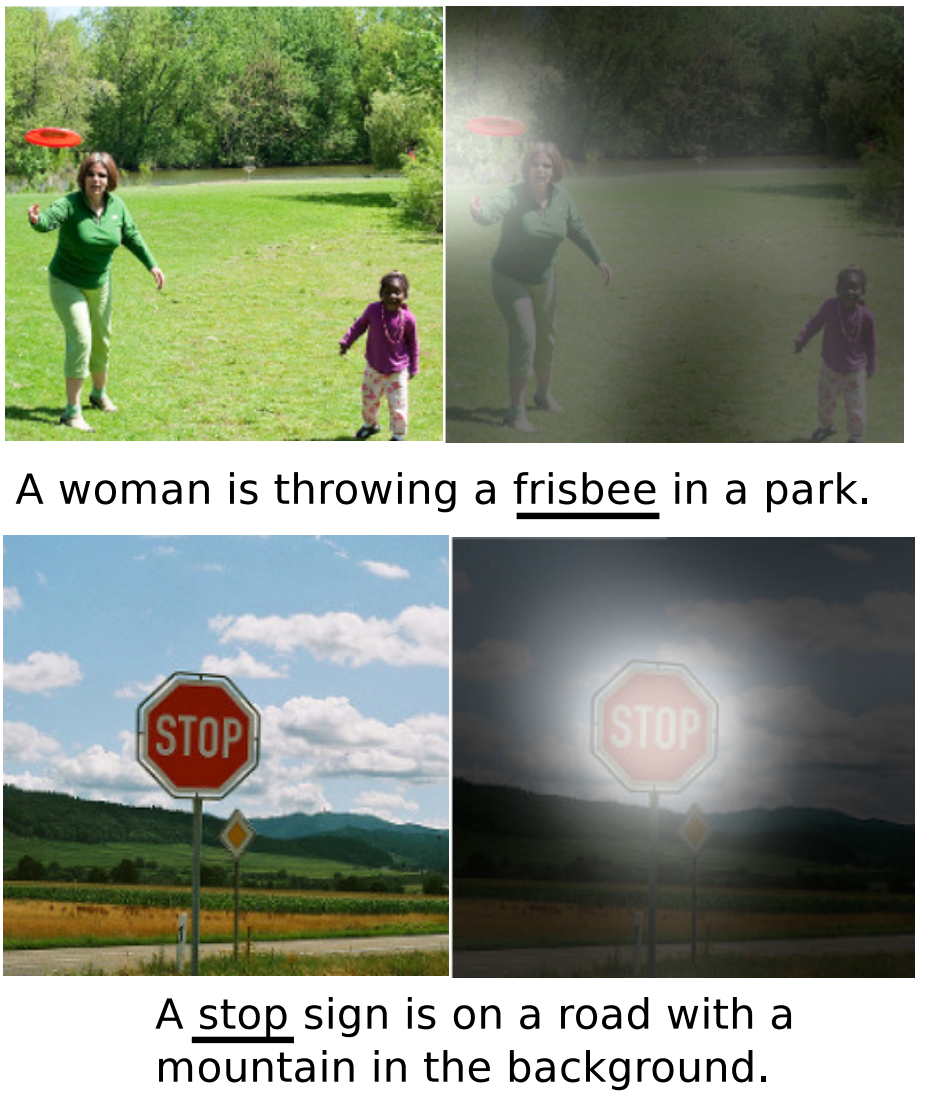
\includegraphics[width=5cm]{plots/attention3.png}
    \caption{Attention for image captioning: the attention mechanism tells the network roughly which pixels to pay attention to when writing the text (Kelvin Xu al. 2015)}
  \end{figure}
}

\section{Transformers}

\begin{vbframe}{Transformers}
  \begin{itemize}
    \item Advanced RNNs have similar limitations as vanilla RNN networks:
    \begin{itemize}
      \item RNNs process the input data sequentially.
     \item Difficulties in learning long term dependency (although GRU or LSTM perform better than vanilla RNNs, they sometimes struggle to remember the context introduced earlier in long sequences).
    \end{itemize}
    \item These challenges are tackled by transformer networks.
    
    \framebreak
    
    \item Transformers are solely based on attention (no RNN or CNN).
    \item In fact, the paper which coined the term \textit{transformer} is called \textit{Attention is all you need}.
    \item They are the state-of-the-art networks in natural language processing (NLP) tasks since 2017.
    \item Transformer architectures like BERT (Bidirectional Encoder Representations from Transformers, 2018) and GPT-3 (Generative Pre-trained Transformer-3, 2020) are pre-trained on a large corpus and can be fine-tuned to specific language tasks.
  \end{itemize}

\framebreak

\begin{center}
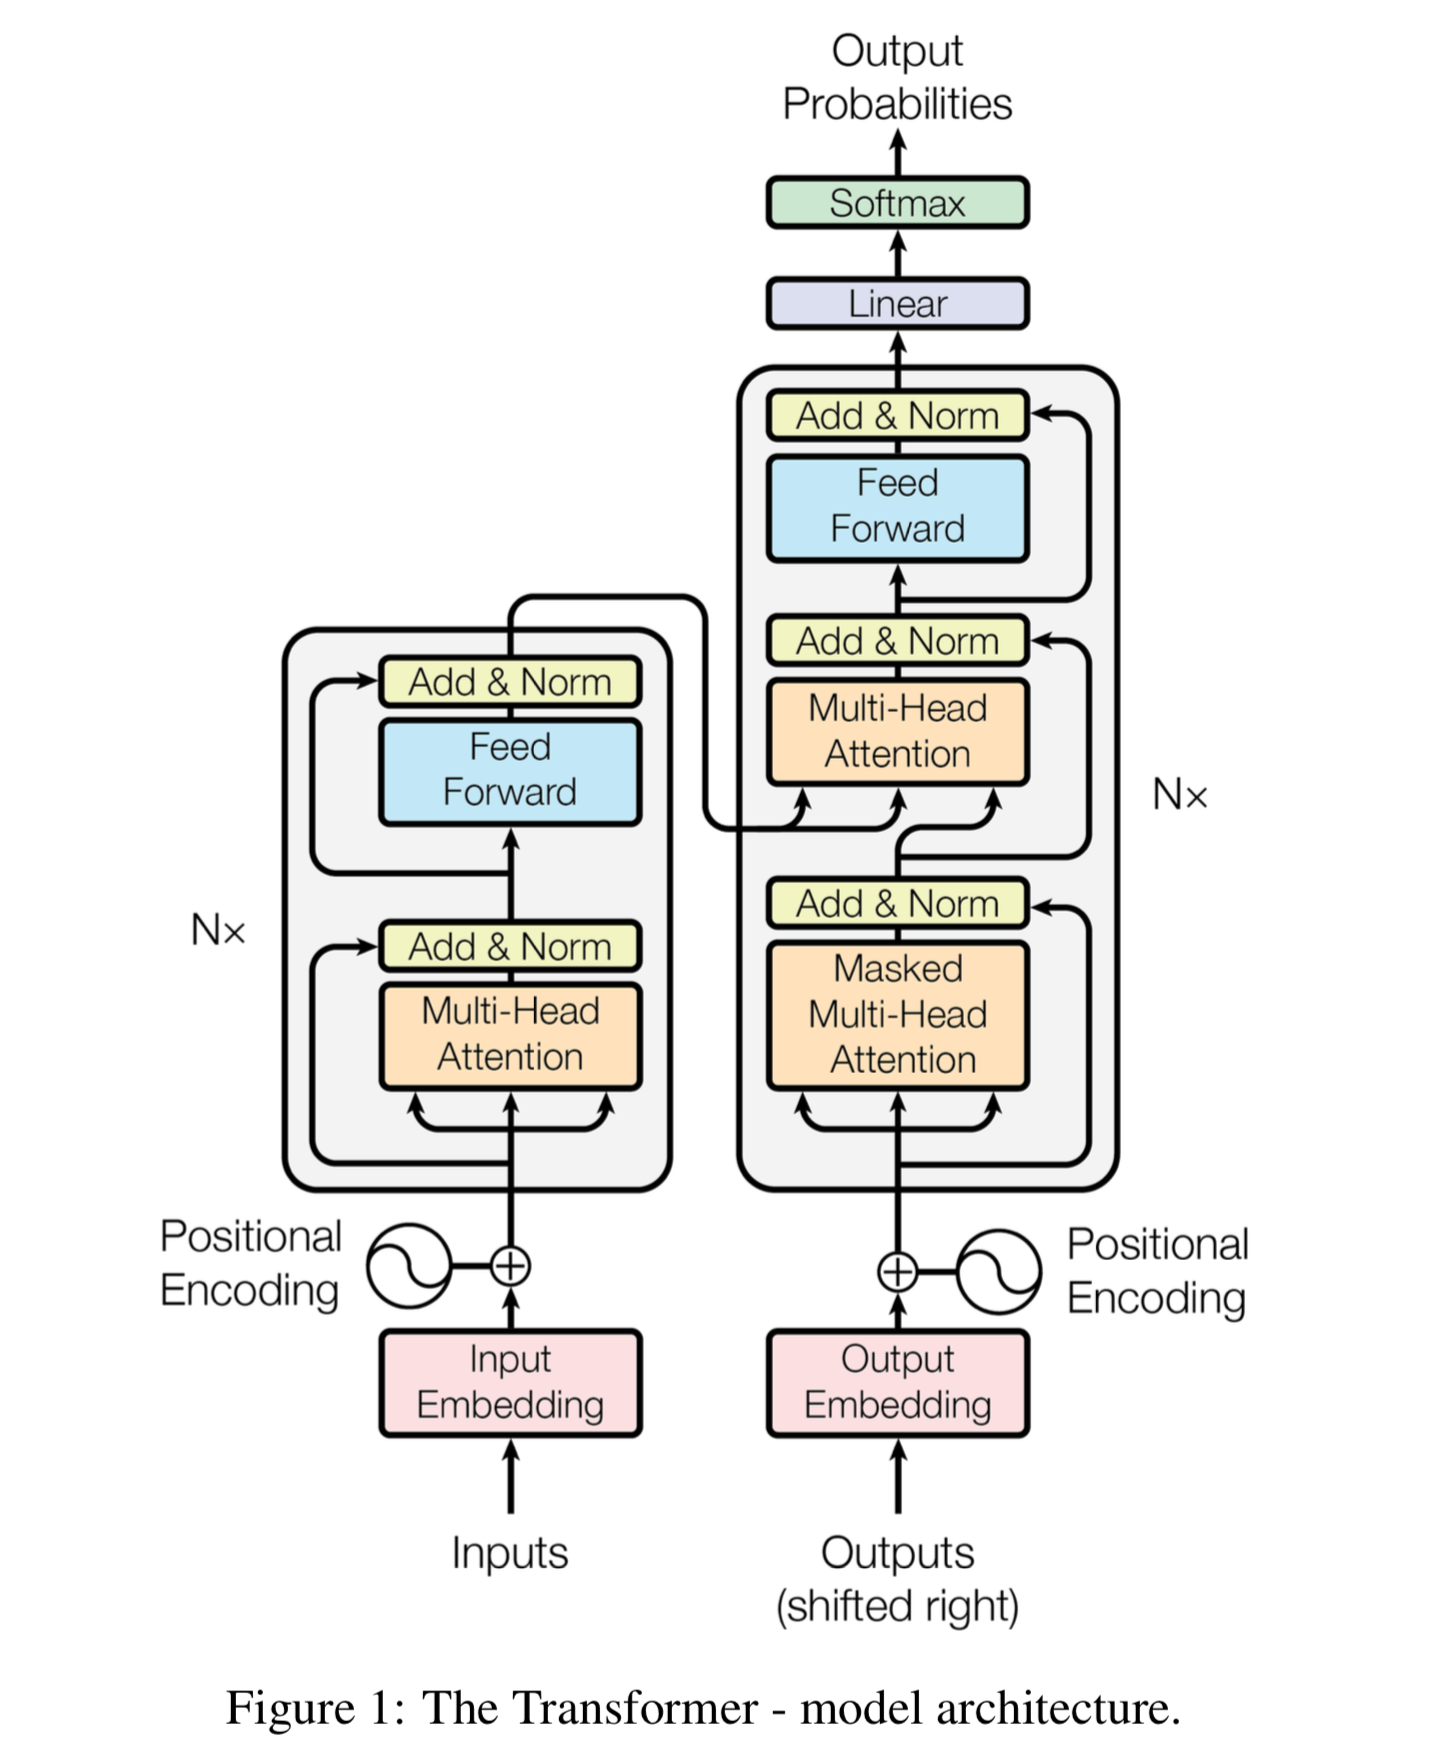
\includegraphics[width=6.5cm]{plots/transformer.png}
\end{center}

\end{vbframe}


%%%%%%%%%%%%%%%%%%%%%%%%%%%%%%%%%%%%%%%%%%%%%%%%%%%%%%%%%%%%%%%%%%

%%%%%%%%%%%%%%%%%%%%%%%%%%%%%%%%%%%%%%%%%%%%%%%%%%%%%%%%%%%%%%%%%%
\section{CNNs or RNNs?}

\begin{frame} {CNNs or RNNs?}
  \begin{itemize}
    \item Historically, RNNs were the default for sequence processing tasks.
    \item However, some families of CNNs (especially those based on Fully Convolutional Networks (FCNs)) \textit{can} be used to process variable-length sequences such as text or time-series data.
    \item If a CNN doesn't contain any fully-connected layers, the total number of weights in the network is independent of the spatial dimensions of the input because of weight-sharing in the convolutional layers.
    \item Recent research [Bai et al. , 2018] indicates that such convolutional architectures, so-called Temporal Convolutional Networks (TCNs), can outperform RNNs on a wide range of tasks.
    \item A major advantage of TCNs is that the entire input sequence can be fed to the network at once (as opposed to sequentially).
    % \item Surprisingly, the TCNs can model long-range dependencies in the inputs even better than recurrent architectures!
  \end{itemize}
\end{frame}

\begin{frame} {CNNs or RNNs?}
  \begin{figure}
      \centering
      \scalebox{1}{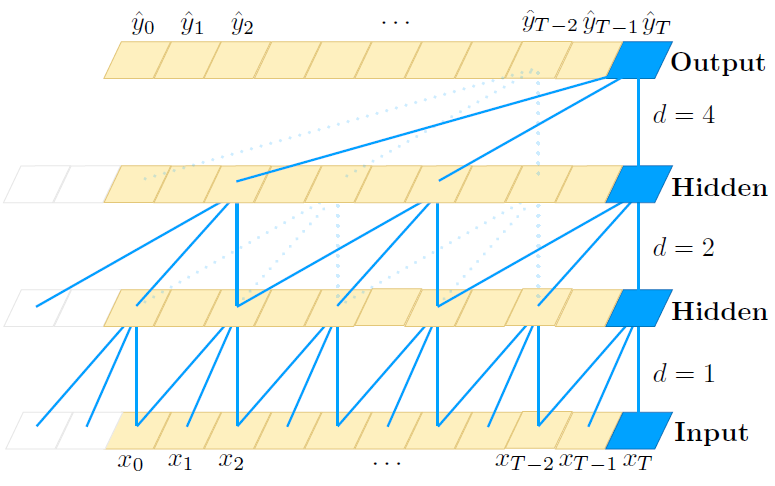
\includegraphics{plots/tcn2.png}}
      \caption{\footnotesize{A TCN (we have already seen this in the CNN lecture!) is simply a variant of the one-dimensional FCN which uses a special type of dilated convolutions called \textbf{causal dilated} convolutions.}}
  \end{figure}
\end{frame}


%\begin{frame} {CNNs or RNNs?}
%  \begin{figure}
%      \centering
%      \scalebox{1}{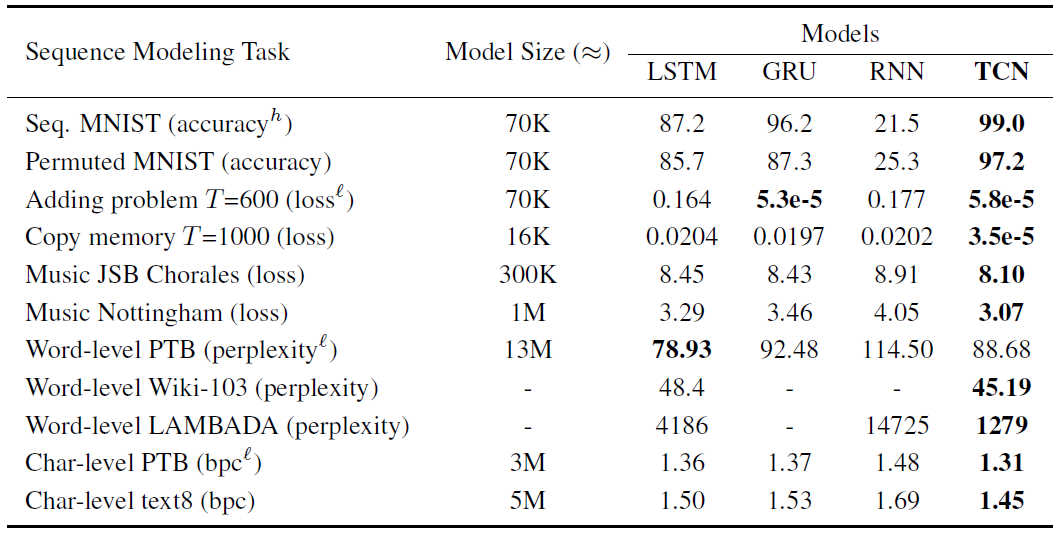
\includegraphics{plots/tcn1.png}}
%      \caption{\footnotesize{Evaluation of TCNs and recurrent architectures on a wide range of sequence modelling tasks. $^h$ means higher is better and ${}^\ell$~ means lower is better. Note: To make the comparisons fair, all models have roughly the same size (for a given task) and the authors used grid search to find good hyperparameters for the recurrent architectures.}}
%  \end{figure}
%\end{frame}


%\begin{frame}{Summary}
%\begin{itemize}
%\item RNNs are specifically designed to process sequences of varying lengths. 
%\item  For that recurrent connections are introduced into the network structure.
%\item The gradient is calculated by backpropagation through time.
%\item  An LSTM replaces the  simple hidden neuron by a complex system consisting of cell state, and forget, input, and output gates.
%\item An RNN can be used as a language model, which can be improved by word-embeddings.
%\item Different advanced types of RNNs exist, like Encoder-Decoder architectures and bidirectional RNNs.$^1$
%\end{itemize}
%
%\vspace{8mm}
%\tiny{1. A bidirectional RNN processes the input sequence in both directions (front-to-back and back-to-front).}
%
%\end{frame}

%%%%%%%%%%%%%%%%%%%%%%%%%%%%%%%%%%%%%%%%%%%%%%%%%%%%%%%%%%%%%%%%%%
%%%%%%%%%%%%%%%%%%          REFERENCES          %%%%%%%%%%%%%%%%%%
%%%%%%%%%%%%%%%%%%%%%%%%%%%%%%%%%%%%%%%%%%%%%%%%%%%%%%%%%%%%%%%%%%
\begin{vbframe}
\frametitle{References}
\footnotesize{
\begin{thebibliography}{99}
%%%%%%%%%%%%%%%%%%%%%%%%%%%%%%%%%%
\bibitem[Ian Goodfellow et al., 2016]{1} Ian Goodfellow, Yoshua Bengio and Aaron Courville (2016)
\newblock Deep Learning
\newblock \emph{\url{http://www.deeplearningbook.org/}}
%%%%%%%%%%%%%%%%%%%%%%%%%%%%%%%%%%
\bibitem[Oriol Vinyals et al., 2014]{2} Oriol Vinyals, Alexander Toshev, Samy Bengio and Dumitru Erhan (2014)
\newblock Show and Tell: A Neural Image Caption Generator
\newblock \emph{\url{https://arxiv.org/abs/1411.4555}}
%%%%%%%%%%%%%%%%%%%%%%%%%%%%%%%%%%
\bibitem[Alex Graves, 2013]{3} Alex Graves (2013)
\newblock Generating Sequences With Recurrent Neural Networks
\newblock \emph{\url{https://arxiv.org/abs/1308.0850}}
%%%%%%%%%%%%%%%%%%%%%%%%%%%%%%%%%%
\bibitem[Namrata Anand and Prateek Verma, 2016]{4} Namrata Anand and Prateek Verma (2016)
\newblock Convolutional and recurrent nets for detecting emotion from audio data
\newblock \emph{\url{http://cs231n.stanford.edu/reports/2015/pdfs/Cs_231n_paper.pdf}}
%%%%%%%%%%%%%%%%%%%%%%%%%%%%%%%%%%
\bibitem[Gabriel Loye, 2019]{5} Gabriel Loye (2019)
\newblock Attention Mechanism
\newblock \emph{\url{https://blog.floydhub.com/attention-mechanism/}}
%%%%%%%%%%%%%%%%%%%%%%%%%%%%%%%%%%
\bibitem[Andrew Owens et al., 2016]{6} Andrew Owens, Phillip Isola, Josh H. McDermott, Antonio Torralba, Edward H. Adelson and  William T. Freeman (2015)
\newblock Visually Indicated Sounds
\newblock \emph{\url{https://arxiv.org/abs/1512.08512}}
%%%%%%%%%%%%%%%%%%%%%%%%%%%%%%%%%%
%%%%%%%%%%%%%%%%%%%%%%%%%%%%%%%%%%
\bibitem[Andrej Karpathy., 2015]{7} Andrej Karpathy (2015)
\newblock The Unreasonable Effectiveness of Recurrent Neural Networks
\newblock \emph{\url{http://karpathy.github.io/2015/05/21/rnn-effectiveness/}}
% \bibitem[Devlin et al., 2018]{7} Jacob Devlin, Ming-Wei Chang, Kenton Lee, Kristina Toutanova (2018)
% \newblock BERT: Pre-training of Deep Bidirectional Transformers for Language Understanding
% \newblock \emph{\url{https://arxiv.org/abs/1810.04805}}
%%%%%%%%%%%%%%%%%%%%%%%%%%%%%%%%%%
\bibitem[Kelvin Xu al., 2016]{8} Kelvin Xu, Jimmy Ba, Ryan Kiros, Kyunghyun Cho, Aaron C. Courville, Ruslan Salakhutdinov, Richard S. Zemel and  Yoshua Bengio (2015)
\newblock Show, Attend and Tell: Neural Image Caption Generation with Visual Attention
\newblock \emph{\url{https://arxiv.org/abs/1502.03044}}
%%%%%%%%%%%%%%%%%%%%%%%%%%%%%%%%%%
\bibitem[Bai et al., 2018]{9} Shaojie Bai, J. Zico Kolter, Vladlen Koltun (2018)
\newblock An Empirical Evaluation of Generic Convolutional and Recurrent Networks for Sequence Modeling
\newblock \emph{\url{https://arxiv.org/abs/1803.01271}}
%%%%%%%%%%%%%%%%%%%%%%%%%%%%%%%%%%
\bibitem[Weng 2018]{10} Lilian Weng (2018)
\newblock Attention? Attention!
\newblock \emph{\url{https://lilianweng.github.io/lil-log/2018/06/24/attention-attention.html}}
%%%%%%%%%%%%%%%%%%%%%%%%%%%%%%%%%%
\end{thebibliography}
}
\end{vbframe}
%%%%%%%%%%%%%%%%%%%%%%%%%%%%%%%%%%%%%%%%%%%%%%%%%%%%%%%%%%%%%%%%%%
%%%%%%%%%%%%%%%%%%%%%%%%%%%%%%%%%%%%%%%%%%%%%%%%%%%%%%%%%%%%%%%%%%

\endlecture
\end{document}